%% Template Elsevier for Neuroimage

%% Use the option review to obtain double line spacing
%\documentclass[authoryear,preprint,review,12pt]{elsarticle}
\documentclass[authoryear,3p]{elsarticle}
\usepackage{natbib}
\usepackage{amsmath}
%\usepackage{lineno}
\usepackage{hyperref}
\usepackage{amssymb}
\usepackage{amsfonts}
\usepackage{graphicx}
\journal{Neuroimage}
%\usepackage{color} 

\begin{document}

% Title must be 150 words or less
\begin{frontmatter}
\title{Point-by-point response to the reviews of the manuscript NIMG-15-3295}


\author[label0,label1,label2]{Pierre Bellec\corref{cor1}}
\address[label0]{The Neuro Bureau}
\address[label1]{Centre de Recherche de l'Institut Universitaire de G\'eriatrie de Montr\'eal, Montr\'eal, CA}
\address[label2]{D\'epartement d'Informatique et de Recherche Op\'erationnelle, Universit\'e de Montr\'eal, Montr\'eal, CA}

\cortext[cor1]{Corresponding authors.}

\ead{pierre.bellec@criugm.qc.ca}
\ead[url]{bellec.simexp-lab.org}

\author[label0,label3]{Carlton Chu}
\address[label3]{Google DeepMind, London, UK}
\ead{carltonchu1@gmail.com}

\author[label0,label1,label4]{Fran\c{c}ois Chouinard-Decorte}
\address[label4]{Integrated Program in Neuroscience, McGill University, Montreal, CA}
\ead{francois.chouinard@gmail.com}

\author[label0,label1,label5]{Yassine Benhajali}
\address[label5]{D\'epartement d'Anthropologie, Universit\'e de Montr\'eal, Montr\'eal, CA}
\ead{yanamarji@gmail.com}

\author[label0,label6]{Daniel S. Margulies}
\address[label6]{Max Planck Research Group for Neuroanatomy \& Connectivity, Max Planck Institute for Human Cognitive and Brain Sciences, Leipzig, Germany}
\ead{margulies@cbs.mpg.de}

\author[label0,lab7,lab8]{R. Cameron Craddock\corref{cor1}}
\address[lab7]{Computational Neuroimaging Laboratory, Center for Biomedical Imaging and Neuromodulation, Nathan S. Kline Institute for Psychiatric Research, Orangeburg, NY, USA}
\address[lab8]{Center for the Developing Brain, Child Mind Institute, New York, NY, USA}
\ead{ccraddock@nki.rfmh.org}
\ead[url]{computational-neuroimaging-lab.org}

\begin{abstract} This is a point-by-point response to the comments of the reviewers for manuscript NIMG-15-3295. We would like to thank both reviewers for their constructive feedback. All changes have been highlighted in the revised manuscript. 
\end{abstract}

\end{frontmatter}


\section{Responses to reviewer 1}


\begin{quote}
$\blacktriangleright$\emph{1. Well, after reading the paper I'd say only one thing: well done. I could follow what you have done, it's described in enough details to be useful - I have therefore only one recommendation for the editor: accept.
Dr Cyril Pernet. }
\end{quote}

Thank you.

\section{Responses to reviewer 2}

\begin{quote}
$\blacktriangleright$\emph{1. The authors document three pre-processing pipelines applied to the ADHD-200 dataset. The work is valuable, and I commend the authors on sharing these pre-processed versions of the ADHD-200 data with the scientific community.} 
\end{quote}

Thank you. 

\begin{quote}
$\blacktriangleright$\emph{2. Regarding quality control, the NIAK pipeline output was carefully inspected to ensure that the pipeline itself worked properly. For example, parameter adjustments were made to improve registration in cases where the registration was poor. It appears that similar quality control, focusing on the pipeline performance (not raw data quality), was \emph{not} done for the Athena and Burner pipelines. Is this correct? If so, why not? I do not see any justification for accepting a pre-processing pipeline that might take good raw data and produce bad pre-processed data. The pre-processing pipeline is under the researcher's control, and it should be required to operate correctly. Note that I agree with your decision and reasoning not to exclude poor quality raw data. Raw data quality cannot always be fully controlled by the researcher, and low quality raw data must sometimes be accepted (eg: with difficult participant populations). Please clarify this issue.} 
\end{quote}

The reviewer is correct. In our original release of the ADHD200 preprocessed sample, no systematic visual assessment of brain registration had been implemented for the Athena pipeline. The main reason was the time constraints of the competition. We have implemented a systematic visual review of T1-template and T1-BOLD registrations for both NIAK and Athena, using an assessment protocol that is currently under development\footnote{\url{https://github.com/SIMEXP/niak_manual/raw/master/qc_manual_v1.0/qc_manual_niak.pdf}}. The reports for quality control have been made publicly available for Athena\footnote{\url{http://simexp.github.io/adhd200_qc_athena/index.html}} and NIAK\footnote{\url{http://simexp.github.io/adhd200_qc_niak/index.html}}. We have also released a spreadsheet including the QC status for each dataset, marked either \texttt{Fail}, in the presence of a major issue, or \texttt{Pass}. 
\par 
A subset of 220 subjects was graded independently by two raters, and the Cohen's kappa agreement was high (81\%) between them. The final status of a processed dataset was \texttt{Fail} if it was marked as such by one of the rater. The remaining 745 subjects were graded only once by one of the raters. In total, we evaluated 1165 subjects (accounting for 200 subjects evaluated twice), times 2 modalities, times 2 pipelines, for a grand total of $4740$ visual assessments of coregistration quality. The failure rate for Athena and NIAK were relatively low: 7\% and 5.2\%, respecively. We are planning to implement a more detailed evaluation of the registration performance as well the quality of raw data in follow up publications. 

\begin{quote}
$\blacktriangleright$\emph{3. page 2, line 9: Are the 26 "unknown" subjects from the Brown University site? If so, their diagnoses are known to the researchers who collected those data, but those diagnoses have not been publicly released. It would be clearer to describe these 26 as "diagnoses not publicly released" rather than "unknown". Similarly for page 3, line 46.}
\end{quote}

Fixed (l. XX-XX). 

\begin{quote}
$\blacktriangleright$\emph{4. page 2, lines 31-32: structure error in sentence, missing "and" ?). 
}
\end{quote}

Fixed (l. XX-XX).

\begin{quote}
$\blacktriangleright$\emph{5. page 3, line 65: missing closing parenthesis}
\end{quote}

Fixed (l. XX-XX).

\begin{quote}
$\blacktriangleright$\emph{6. Oxford comma used in some places but not others, better style if consistent throughout}
\end{quote}

We have edited the document to use the Oxford comma, consistently.

\begin{quote}
$\blacktriangleright$\emph{7. Figure 1: "An example of an individual map is presented". I do not see a single subject map, just the average and standard deviation maps.}
\end{quote}

Fixed (l. XX-XX). 

\begin{quote}
$\blacktriangleright$\emph{8.  Page 9, line 166: "For each data type a mean and standard deviation image ...": Does each data type mean just {s-MRI, rs-MRI} or does it also include the other derivative images (eg: fALFF maps, etc.)?}
\end{quote}

``Each data type'' includes all derivatives. The paragraph was edited to clarify this (l. XX-XX). 

\begin{quote}
$\blacktriangleright$\emph{9. Page 9, line 166-171: Were the z-score calculations done on the raw data, preprocessed data, or both?}
\end{quote}

The z-score calculations were done on preprocessed data, registered in stereotaxic space. We edited the paragraph to clarify this (l. XX-XX). 

\begin{quote}
$\blacktriangleright$\emph{10. Page 11, line 260-261: Erroneous symbols (eg: upside down ! and ?)}
\end{quote}

Fixed (l.XX-XX).

\section{Responses to reviewer 3}

\begin{quote}
$\blacktriangleright$\emph{1. The efforts from Neuro Bureau described were extremely important in making the ADHD200 Competition a relative success, as many participants used, at least in part, these intermediate results to assist their work. A large number of publications are reported in the Conclusions section, though it is not immediately apparent to what extent each of these papers hinged on the datasets / intermediate results described here.  It would be very beneficial to provide some additional details (case examples would suffice) on how the data have been used rather than simply providing a bulk citation list. 
}
\end{quote}

We added a paragraph at the beginning of "usage recommendation" (lines XX-XX) where we describe a few works that used ADHD-200 preprocessed. The vast majority of these publications aimed at predicting clinical labels from brain data, either structurally with Burner or functionally with Athena/NIAK, or both. We pointed at different papers based on the derivatives they used. In addition, in the discussion (lines XX-XX), we referred to a handful of studies that combined ADHD-200 preprocessed with data samples from unrelated fields to evaluate statistical models, which we see as an important direction enabled by the ADHD-200 preprocessed initiative. 


\begin{quote}
$\blacktriangleright$\emph{2. While the ADHD-200 Preprocessed Repository is of high value, as evidenced by a large number of downloads, there is some concern about the ongoing relevance of this publication, now several years after the initial processing was performed and the ADHD200 challenge was held. The authors state that they have no plans to expand or update the release, and instead only state that they hope it will "continue to serve as a legacy benchmark dataset."  I agree that there is utility in maintaining a benchmark dataset (with multiple publications / results against which new efforts can be compared). However, if this is the goal, then perhaps the authors might also collate and host (alongside the data) some of the benchmark "results" using these methods to make the use of the data for this purpose even easier?  A minimal solution might be including web links from NITRC to results of the ADHD Global Competition, and to papers that used the preprocessed dataset.
}
\end{quote}

We added a reference in the discussion (l. XXX) to the ADHD200 preprocessed Mendeley library (https://www.mendeley.com/groups/4198361/adhd-200-preprocessed/), an online collection of the publications that used the ADHD200. This resource is being regularly updated by the laboratory of Dr Craddock. 

\begin{quote}
$\blacktriangleright$\emph{3. In addition, it would be useful if the authors could provide evidence and further discussion of the long-term relevance of this dataset. For example, how has the number of downloads changed since the ADHD200 Competition ended?  Are the forums still be used?  Are there research groups actively working with these processed data now?}
\end{quote}
\begin{figure}[!t]
\begin{center}
  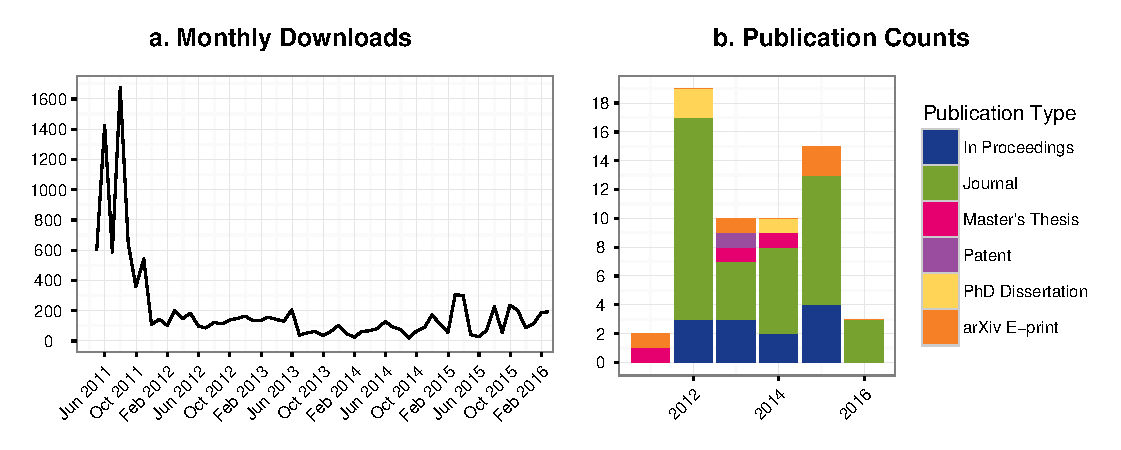
\includegraphics[width=\linewidth]{impact_stats}
  \caption{Statistics on download and citations of the ADHD200 preprocessed initiative.}
  \label{fig:usage}
\end{center}
\end{figure}

Although there was clearly a peak in usage around the ADHD-200 Global competition, there has been a sustained amount of downloads and publications since then (Figure \ref{fig:usage}), which we take as a demonstration of a long-term interest from the community in this resource.  We added this point in the discussion (l. XX-XX).


\begin{quote}
$\blacktriangleright$\emph{4. In general, the Discussion ("5. Conclusions") is very light, and it would be helpful to have more of an exposition on the potential forward value of the repository - how unique is it?  How important does it seem to be for ADHD research?  What are the other uses?  Some of this is touched on in Section 4, but a bit more of a forward-looking vision for the repository would be helpful.  Relatedly, do the authors envision any mechanism by which other individuals might add preprocessed results from different processing tools / pipelines to the existing data?
}
\end{quote}

Thanks for the suggestions. We have expanded the discussion, as suggested, in two ways. First, we better emphasized the type of usage that have appeared in the literature (see our response to point 1 above). This helps show how the ADHD-200 prepocessed sample has been used outside of the traditional brain imaging community, and has started to be adopted by researchers doing core statistics, signal processing and machine learning research. We believe that to be quite unique and a potentially important development in the field. Second, we added a paragraph discussing the value of having two independent processing pipelines availables in the sample, which has not yet been exploited. To the best of our knowledge, this is a feature unique to ADHD-200 Preprocessed, which we emphasized in the abstract. Third, we have discussed the ABIDE preprocessed initiative\footnote{\url{http://preprocessed-connectomes-project.org/abide/}}, which builds on the lessons learned by releasing ADHD-200 Preprocessed. In this new release, we were able to include more tools, better quality control, as well as better harmonization of data organization across tools. Recruitment of contributions as been implemented openly, notably during public hackathons. We have added these points to the discussion (l. XX-XX).   

\begin{quote}
$\blacktriangleright$\emph{5. Additional information could be provided that would be helpful to researchers interested in working with preprocessed results from the repository. In particular, what are the limitations and assumptions of each processing stream?  What are seen as the fundamental differences between the NIAK cleaned rs-fMRI volumes and the Athena volumes? There must have been some justification for providing both, but it is not entirely clear here, other than to say users can decide what they want to use; if one goal is to target non-fMRI scientists, then further explication of these differences would be helpful. It would be even more helpful to provide an explicit comparison between the rs-fMRI data from NIAK and Athena.  Just how similar are the processed rs-fMRI image series?  The authors should also explicitly note the limitations of working with preprocessed data (i.e., results depend somewhat on the particular registration strategy used, etc.), and describe if it is possible for users
to go back to raw data (still available?), modify the processing scripts provided, and obtain new intermediate results since this would seem to be a common use case, especially as new methods are developed.
}
\end{quote}

We added a paragraph in the discussion (l. XX-XX) highlighting some of the key differences in the preprocessing parameters. We also discussed our choices re preprocessing strategies, and how this could be improved. Being an open community initiative, the NeuroBureau welcomes contributions from any interested research group. The NITRC site includes a discussion forum where any interested contributor can reach out to us. Six groups have contributed to our latest initiative, the ABIDE preprocessed, using this approach. The brainhack meeting series (Craddock et al., 2016) has also been instrumental to raise awareness and recruit new contributors. 

\begin{quote}
$\blacktriangleright$\emph{6. Some description of the "Neuro Bureau" would be helpful in the introduction - exactly who is this group, and what is their overall mission?
}
\end{quote}

The Neuro Bureau is a non-profit organization and aimed at facilitating open science grassroots initiatives. See the following website\footnote{\url{http://www.neurobureau.org/mission-statement/}} for the full mission statement. We added these details in the introduction (l. XX-XX).  

\begin{quote}
$\blacktriangleright$\emph{ 7. There is a typo / grammatical error in Section 2 (p. 2) "This registration enables downloads to be tracked for usage statistics users to be contacted..."
}
\end{quote}
Fixed (l. XX). 


\begin{quote}
$\blacktriangleright$\emph{ 
8. There is some redundancy between the description of the contents of the repository (p. 3) and the Introduction (in terms of numbers of subjects, etc.).
}
\end{quote}
We have removed the details on the sample size in terms of clinical category from the introduction, and kept these details in the Section "Contents of the repository". 

\begin{quote}
$\blacktriangleright$\emph{ 
9. Why are the NIAK scripts provided on Github, but others provided in NITRC?}
\end{quote}
Scripts for both releases are now hosted on github. See lines XX and XX. 

\begin{quote}
$\blacktriangleright$\emph{ 
10. A bit more methodological detail should be provided on the ICN time series and spatial maps (p. 8).  Was the spatial regression based on a set of templates/maps?  Which ones?}
\end{quote}
The dual regression procedure was implemented based on a template of 10 intrinsic connectivity networks generated using group ICA by Smith and colleagues (PNAS, 2009). We modified the text to make this more explicit (l. XX-XX). 

\begin{quote}
$\blacktriangleright$\emph{ 
11. There is a missing citation on page 10 (Section 3.3.1).
}
\end{quote}

Fixed (l. XX)


\end{document}
